\RequirePackage{fix-cm}
\documentclass[12pt]{article}
\usepackage[utf8]{inputenc}
\usepackage[T1]{fontenc}
\usepackage[paperwidth=594mm, paperheight=841mm, margin=0mm]{geometry}
\usepackage{helvet}
\renewcommand{\familydefault}{\sfdefault}
\usepackage{amsmath,amssymb}
\usepackage{graphicx}
\usepackage{xcolor}
\usepackage{tikz}
\usepackage{enumitem}
\usepackage{microtype}
\pagestyle{empty}

% ==============================================================================
% ZONA DE EDICION RAPIDA — POSTER JORNADAS DE INVESTIGACION MCI UDP 2026
% Tamaño oficial: A1 Vertical (59,4 x 84,1 cm) | Regla: Maximo 300 palabras
% Edite libremente los textos aqui y recompile en Overleaf (Ctrl + Enter).
% ==============================================================================

\newcommand{\PosterTitulo}{Capas tempranas CNN y Gated Attention buscan clasificar biopsias en un pase}
\newcommand{\PosterEtapaMencion}{Seminario I $\cdot$ Inform\'atica y Telecomunicaciones}
\newcommand{\PosterAutorGuia}{Lucas Vicu\~na Fuenzalida $\cdot$ Profesor gu\'ia: Dr. Jorge E. Zambrano Ibuj\'es}

% --- ZONA 1: PROBLEMA Y ESTADO DEL ARTE ---
\newcommand{\ZonaUnoMensaje}{La supervisi\'on d\'ebil y el recorte en p\'ixeles diluyen el tumor y saturan la memoria.}

\newcommand{\IntroTexto}{%
Una biopsia gigap\'ixel solo tiene etiqueta global por paciente ($Y \in \{0,1\}$). Promediar parches diluye micro-tumores y evaluar miles colapsa la VRAM.%
}

\newcommand{\EstadoArteTexto}{%
En MIL por embebidos, \textit{Gated Attention} filtra ruido en costo lineal $\mathcal{O}(K)$. Aparte, truncar CNNs al 33\thinspace\% ahorra $\sim$60\thinspace\% de c\'omputo sin reentrenar.%
}

\newcommand{\VacioNovedad}{%
Nadie ha formado instancias MIL desde mapas CNN intermedios en un pase junto a Gated Attention sin recortar p\'ixeles.%
}

\newcommand{\ObjetivoGeneral}{%
clasificar biopsias H\&E uniendo sub-regiones de capas CNN intermedias ($\le 33$\thinspace\%) con Gated Attention MIL.%
}

\newcommand{\ObjetivosEspecificos}{%
1) extraer tensores en un pase; 2) reducir canales y ponderar con $\tanh \odot \mathrm{sigm}$; 3) medir AUC, IoU y FLOPs.%
}

% --- ZONA 2: METODO PROPUESTO Y AVANCE A LA FECHA ---
\newcommand{\MetodoMensaje}{Un pase CNN truncado genera sub-regiones filtradas por Gated Attention.}
\newcommand{\MetodoDetalle}{Redes congeladas frente a parches (Sudharshan). Evaluaci\'on por paciente: AUC, F1, IoU y FLOPs.}

\newcommand{\AvanceMensaje}{Verificamos el filtrado del Gated Attention y estructuramos cinco cohortes.}
\newcommand{\AvanceDetalle}{La compuerta $\mathrm{sigm}$ suprime falsos positivos y deja listas BreaKHis (81 IDs), PCam, CRC, MHIST y CAM16.}

% --- ZONA 3: PLAN DE TRABAJO ---
\newcommand{\PlanMensaje}{Al cerrar Seminario II tendremos el pipeline intermedio con Gated-MIL medido ante el baseline.}

% --- PIE: RETROALIMENTACION Y EVENTO ---
\newcommand{\PreguntaUno}{?`Conviene reducir canales del mapa intermedio con proyecci\'on $1\times 1$ o filtro estad\'istico?}
\newcommand{\PreguntaDos}{?`C\'omo incorporar contexto espacial entre sub-regiones manteniendo costo lineal $\mathcal{O}(K)$?}
\newcommand{\PieEvento}{Jornadas de Investigaci\'on del Mag\'ister en Ciencias de la Ingenier\'ia $\cdot$ diciembre de 2026}
\newcommand{\PieFinanciamiento}{Programa Mag\'ister en Ciencias de la Ingenier\'ia $\cdot$ Facultad de Ingenier\'ia y Ciencias UDP}

% ==============================================================================
% PALETA INSTITUCIONAL OFICIAL UDP (Un solo acento + negro y escala de grises)
% ==============================================================================
\definecolor{udpred}{HTML}{DC3239}
\definecolor{udppink}{HTML}{FFE3E4}
\definecolor{udpcoral}{HTML}{F4858A}
\definecolor{udpivory}{HTML}{F6F3EE}
\definecolor{udpink}{HTML}{20242A}
\definecolor{udpfooter}{HTML}{2C3036}
\definecolor{udpmuted}{HTML}{4A4F57}
\definecolor{udpline}{HTML}{D8D5CE}
\definecolor{udpfootgray}{HTML}{B8BEC6}

\newcommand{\fsize}[2]{\fontsize{#1}{#2}\selectfont\spaceskip=0.32em\relax}

\begin{document}
\noindent
\begin{tikzpicture}[x=1cm, y=-1cm, remember picture, overlay, shift={(current page.north west)}, every node/.style={align=left}]

  % --- FONDOS DE ZONAS (coordenadas exactas Guia_Poster_MCI_2026) ---
  \fill[white]     (0, 0)     rectangle (59.40, 84.10);
  \fill[udpred]    (0, 0)     rectangle (59.40, 14.80);
  \fill[udpivory]  (0, 14.80) rectangle (59.40, 46.00);
  \fill[udpfooter] (0, 74.60) rectangle (59.40, 84.10);

  % --- ENCABEZADO INSTITUCIONAL MCI / UDP FIC ---
  \node[anchor=north west, inner sep=0pt, text=white] at (3.00, 2.05) {\fsize{46}{48}\bfseries MCI};
  \draw[white, line width=1.4pt] (7.15, 2.15) -- (7.15, 4.25);
  \node[anchor=north west, inner sep=0pt, text=white, text width=12cm] at (7.65, 2.15) {%
    \fsize{23}{27}\bfseries Mag\'ister en Ciencias\\de la Ingenier\'ia%
  };
  \node[anchor=north west, inner sep=0pt] at (45.40, 2.20) {%
    
\includegraphics[width=11.00cm]{assets/logo_fic_blanco.png}%
  };

  % Titulo principal (<= 2 lineas, 62 pt Bold)
  \node[anchor=north west, inner sep=0pt, text=white, text width=53.40cm] at (3.00, 5.45) {%
    \fsize{61}{69}\bfseries \PosterTitulo\par
  };

  % Etapa, mencion, autor y profesor guia (24 pt)
  \node[anchor=north west, inner sep=0pt, text width=53.40cm] at (3.00, 12.10) {%
    \fsize{24}{28}\textcolor{white}{\textbf{\PosterEtapaMencion}}\textcolor{udppink}{\;$\cdot$\;\PosterAutorGuia}\par
  };

  % ============================================================================
  % ZONA 1: PROBLEMA Y ESTADO DEL ARTE (y = 14.80 .. 46.00 cm)
  % ============================================================================
  \fill[udpred] (3.00, 16.50) rectangle (4.60, 16.72);
  \node[anchor=north west, inner sep=0pt, text=udpred] at (3.00, 17.05) {%
    \fsize{20}{24}\bfseries Problema y estado del arte%
  };
  \node[anchor=north west, inner sep=0pt, text=udpink, text width=53.40cm] at (3.00, 18.10) {%
    \fsize{31}{36}\bfseries \ZonaUnoMensaje\par
  };

  % Columna Izquierda: Introduccion al problema
  \node[anchor=north west, inner sep=0pt, text=udpink] at (3.00, 20.60) {%
    \fsize{26}{30}\bfseries Introducci\'on al problema%
  };
  \node[anchor=north west, inner sep=0pt] at (3.00, 21.90) {%
    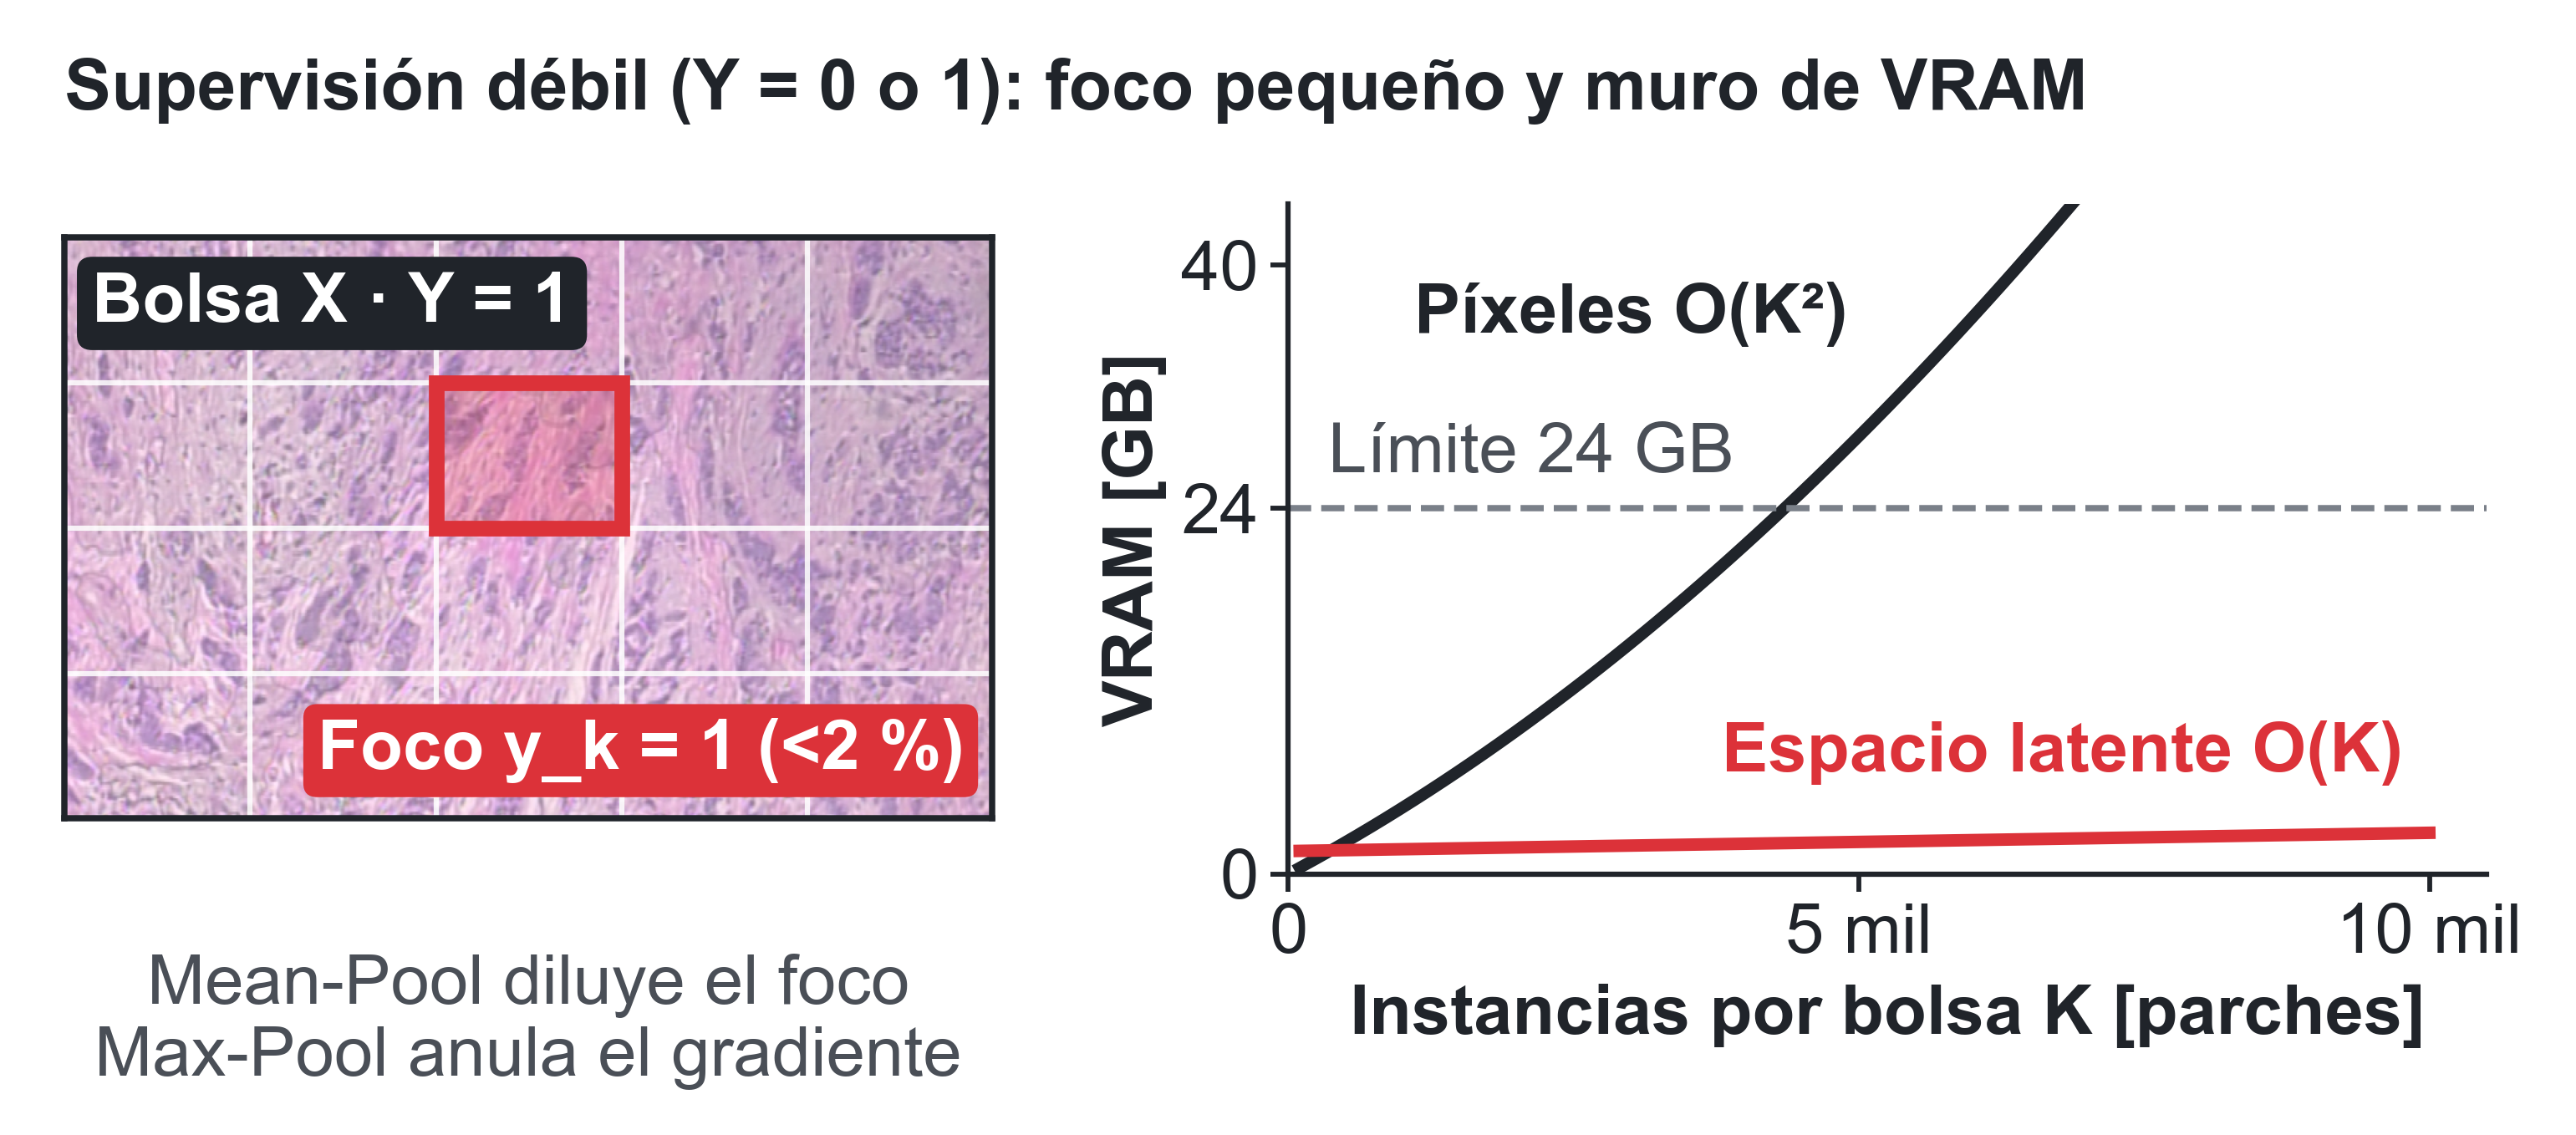
\includegraphics[width=26.10cm, height=11.50cm]{assets/fig1_problema.png}%
  };
  \node[anchor=north west, inner sep=0pt, text=udpink, text width=26.10cm] at (3.00, 33.90) {%
    \fsize{24}{30}\IntroTexto\par
  };

  % Columna Derecha: Estado del arte
  \node[anchor=north west, inner sep=0pt, text=udpink] at (30.30, 20.60) {%
    \fsize{26}{30}\bfseries Estado del arte%
  };
  \node[anchor=north west, inner sep=0pt] at (30.30, 21.90) {%
    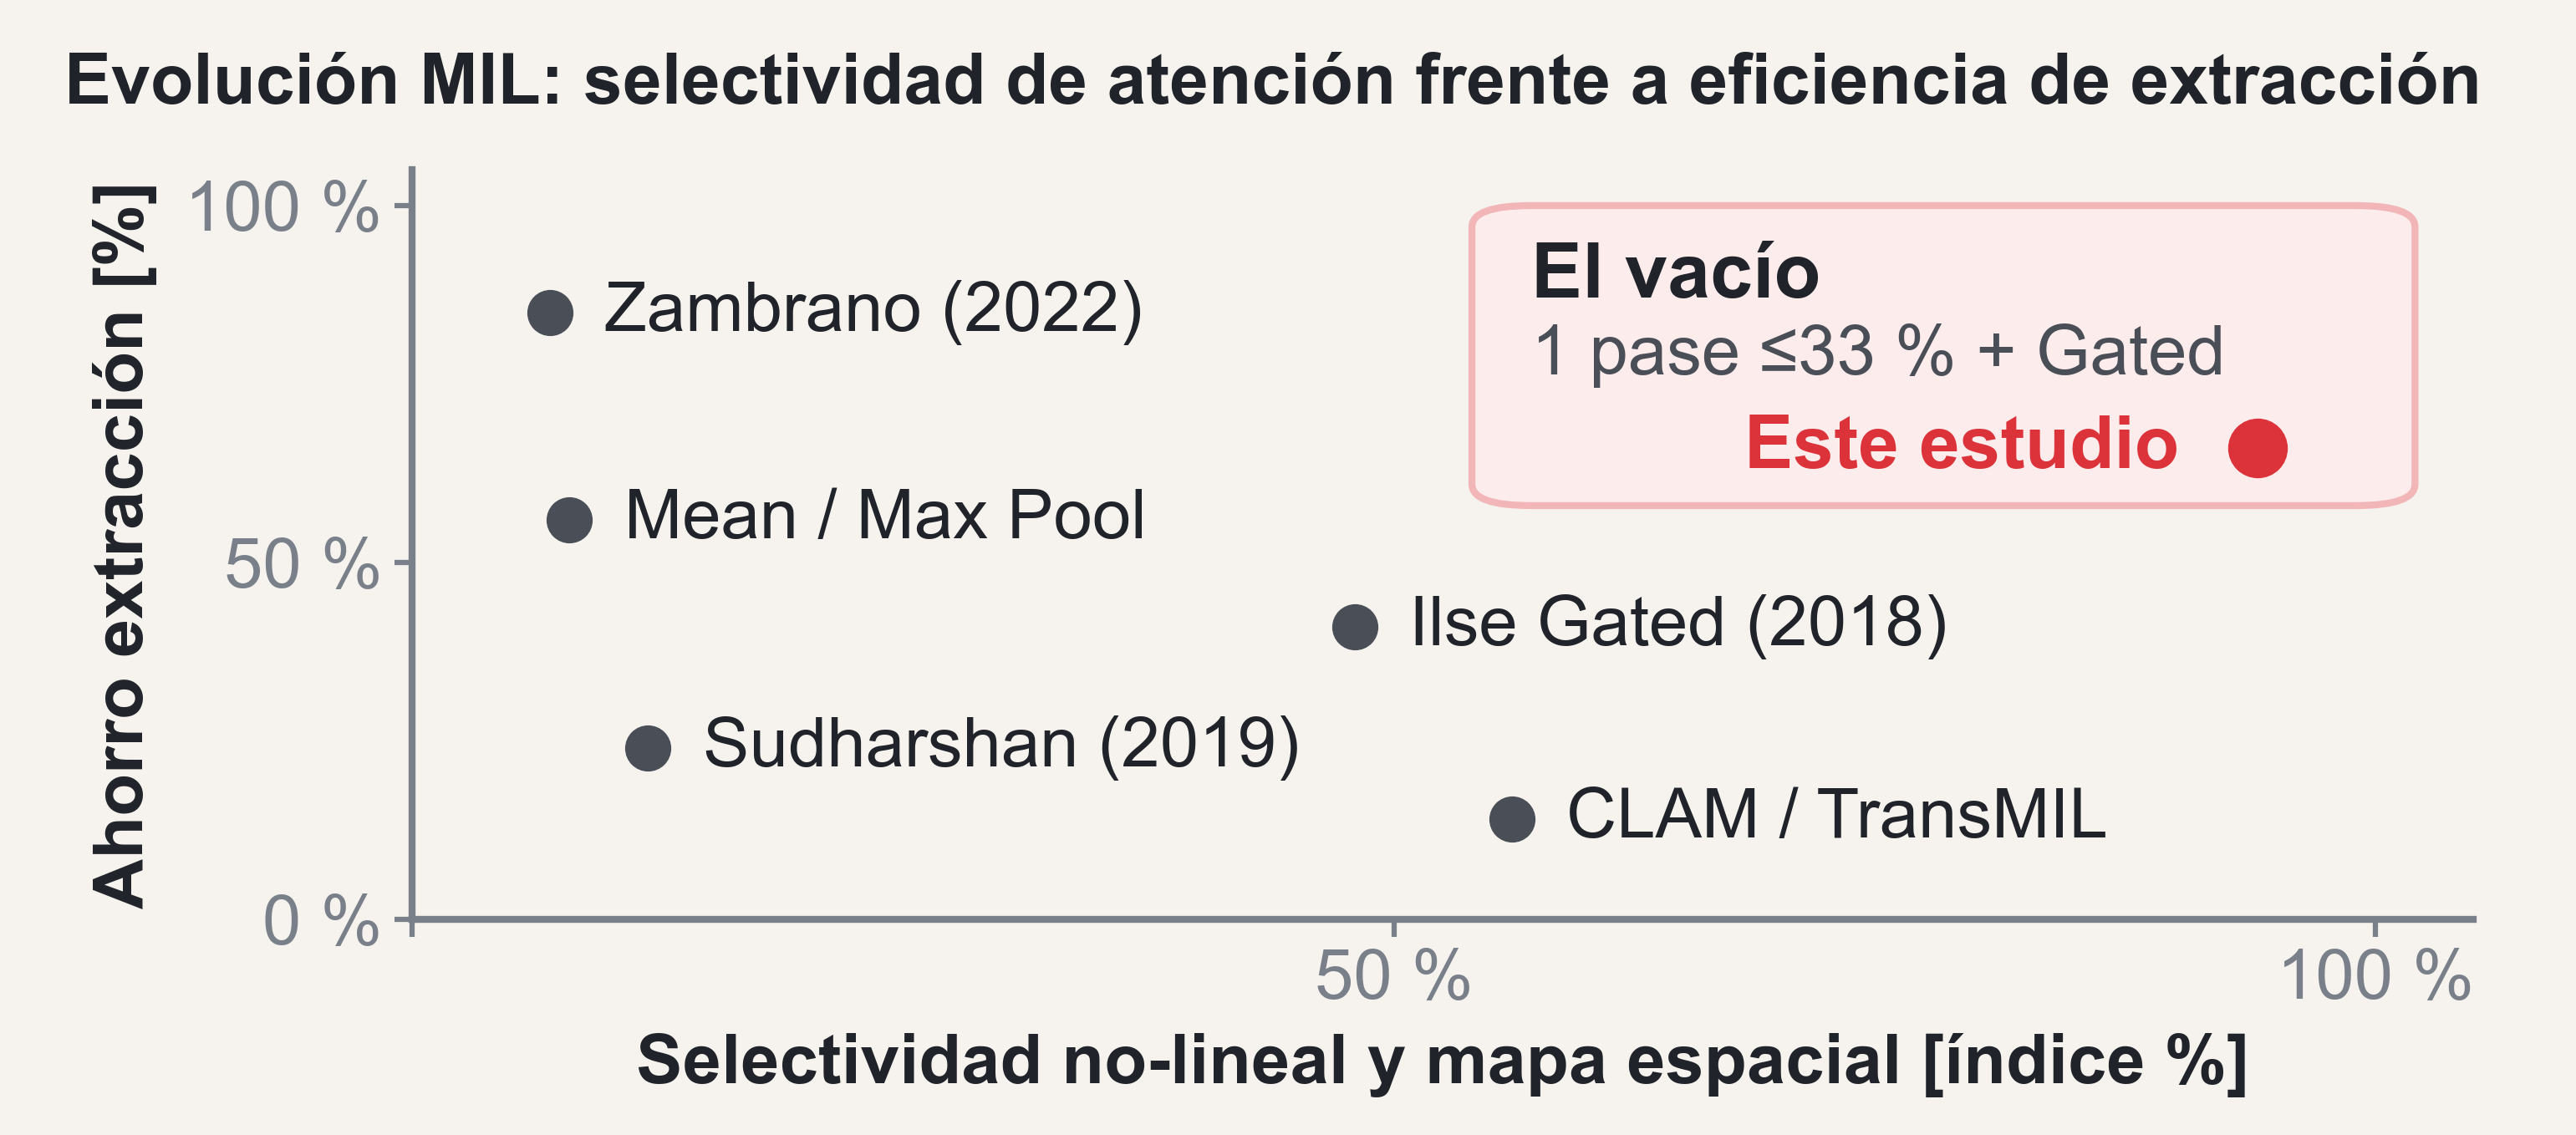
\includegraphics[width=26.10cm, height=11.50cm]{assets/fig2_estado_arte.png}%
  };
  \node[anchor=north west, inner sep=0pt, text=udpink, text width=26.10cm] at (30.30, 33.90) {%
    \fsize{24}{30}\EstadoArteTexto\par
  };

  % Vacio y novedad (con barra vertical roja)
  \fill[udpred] (3.00, 38.60) rectangle (3.30, 44.10);
  \node[anchor=north west, inner sep=0pt, text=udpink] at (4.00, 38.55) {%
    \fsize{26}{30}\bfseries Vac\'io y novedad%
  };
  \node[anchor=north west, inner sep=0pt, text=udpred, text width=25.10cm] at (4.00, 39.80) {%
    \fsize{30}{36}\bfseries \VacioNovedad\par
  };

  % Objetivos
  \node[anchor=north west, inner sep=0pt, text=udpink] at (30.30, 38.55) {%
    \fsize{26}{30}\bfseries Objetivos%
  };
  \node[anchor=north west, inner sep=0pt, text=udpink, text width=26.10cm] at (30.30, 39.80) {%
    \fsize{24}{30}\textbf{General:} \ObjetivoGeneral\\[4pt]
    \textbf{Espec\'ificos:} \ObjetivosEspecificos\par
  };

  % ============================================================================
  % ZONA 2: METODO PROPUESTO Y AVANCE A LA FECHA (y = 46.00 .. 63.40 cm)
  % ============================================================================
  % Izquierda: Metodo
  \fill[udpred] (3.00, 47.50) rectangle (4.60, 47.72);
  \node[anchor=north west, inner sep=0pt, text=udpred] at (3.00, 48.05) {%
    \fsize{20}{24}\bfseries Dise\~no metodol\'ogico propuesto%
  };
  \node[anchor=north west, inner sep=0pt, text=udpink, text width=26.10cm] at (3.00, 49.05) {%
    \fsize{27.5}{33}\bfseries \MetodoMensaje\par
  };
  \node[anchor=north west, inner sep=0pt] at (3.00, 52.00) {%
    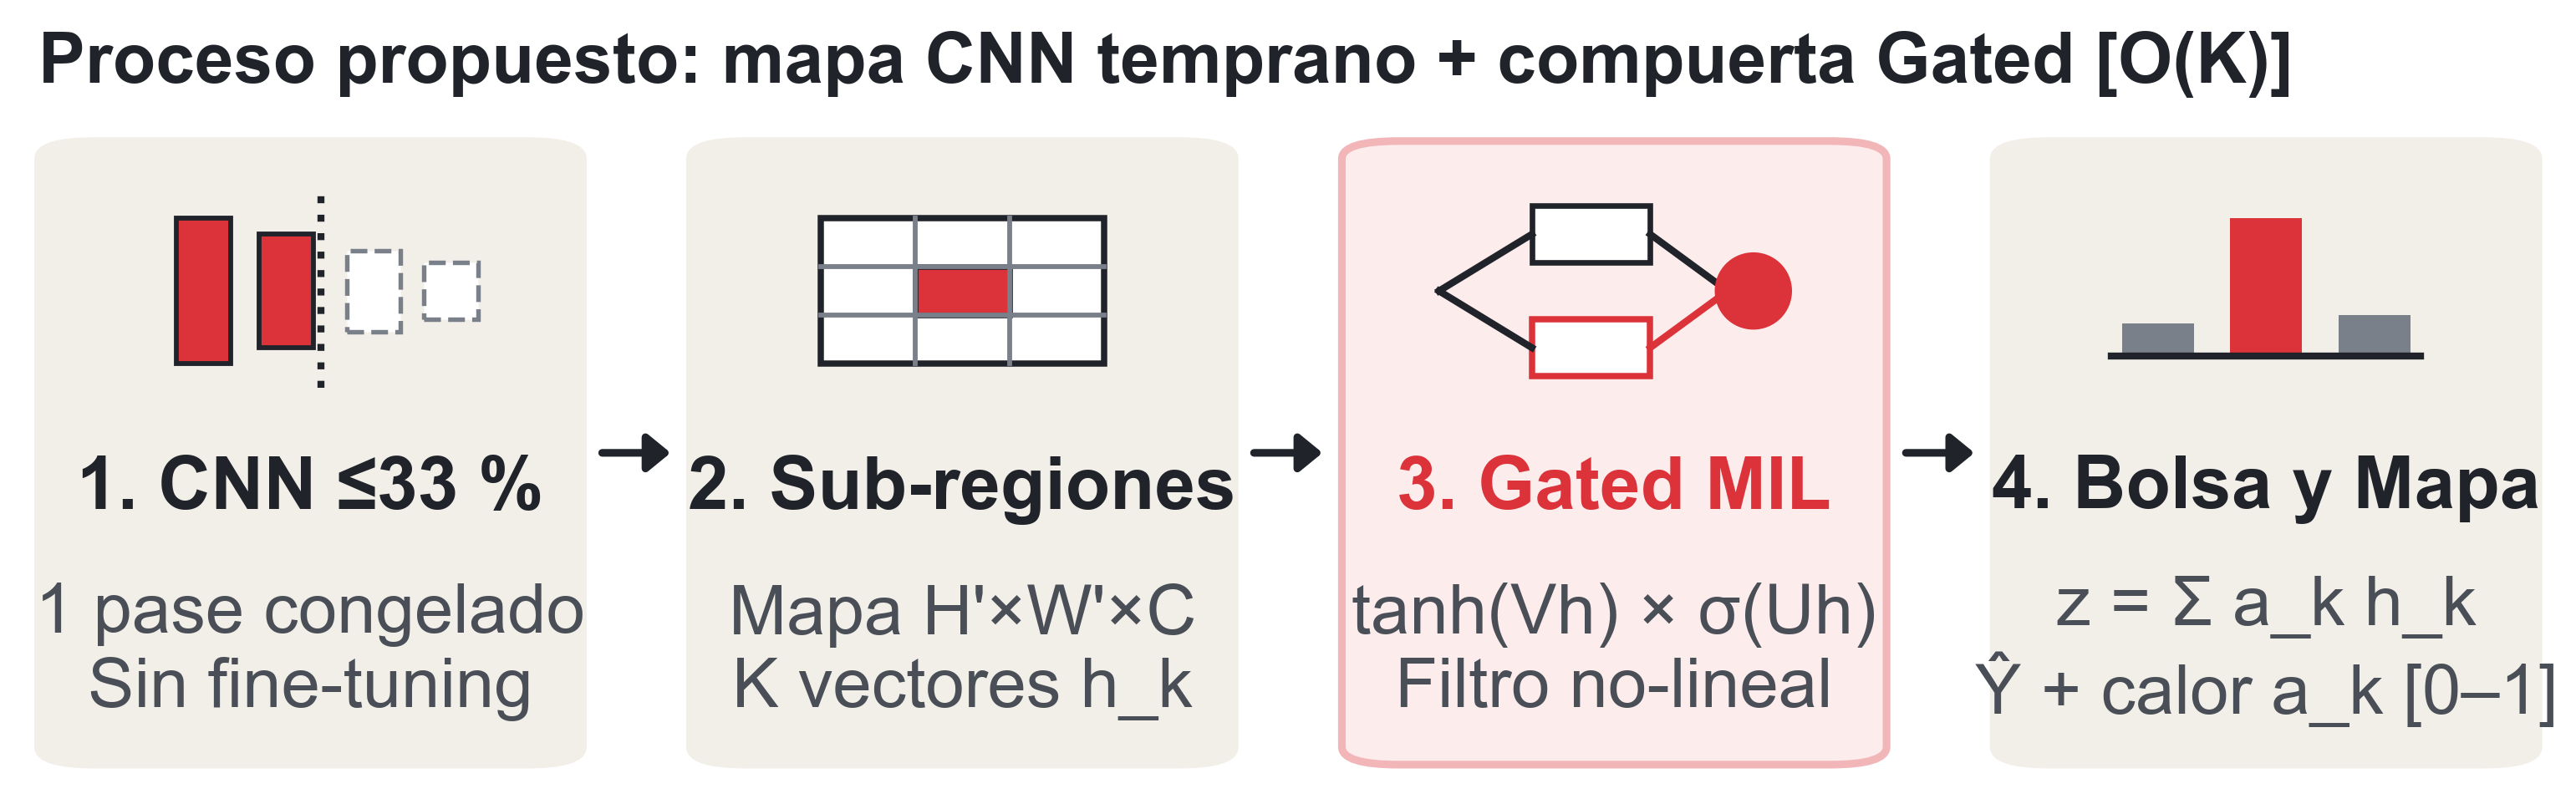
\includegraphics[width=26.10cm, height=8.20cm]{assets/fig3_metodo.png}%
  };
  \node[anchor=north west, inner sep=0pt, text=udpink, text width=26.10cm] at (3.00, 60.60) {%
    \fsize{24}{29}\MetodoDetalle\par
  };

  % Derecha: Avance
  \fill[udpred] (30.30, 47.50) rectangle (31.90, 47.72);
  \node[anchor=north west, inner sep=0pt, text=udpred] at (30.30, 48.05) {%
    \fsize{20}{24}\bfseries Avance a la fecha%
  };
  \node[anchor=north west, inner sep=0pt, text=udpink, text width=26.10cm] at (30.30, 49.05) {%
    \fsize{27.5}{33}\bfseries \AvanceMensaje\par
  };
  \node[anchor=north west, inner sep=0pt] at (30.30, 52.00) {%
    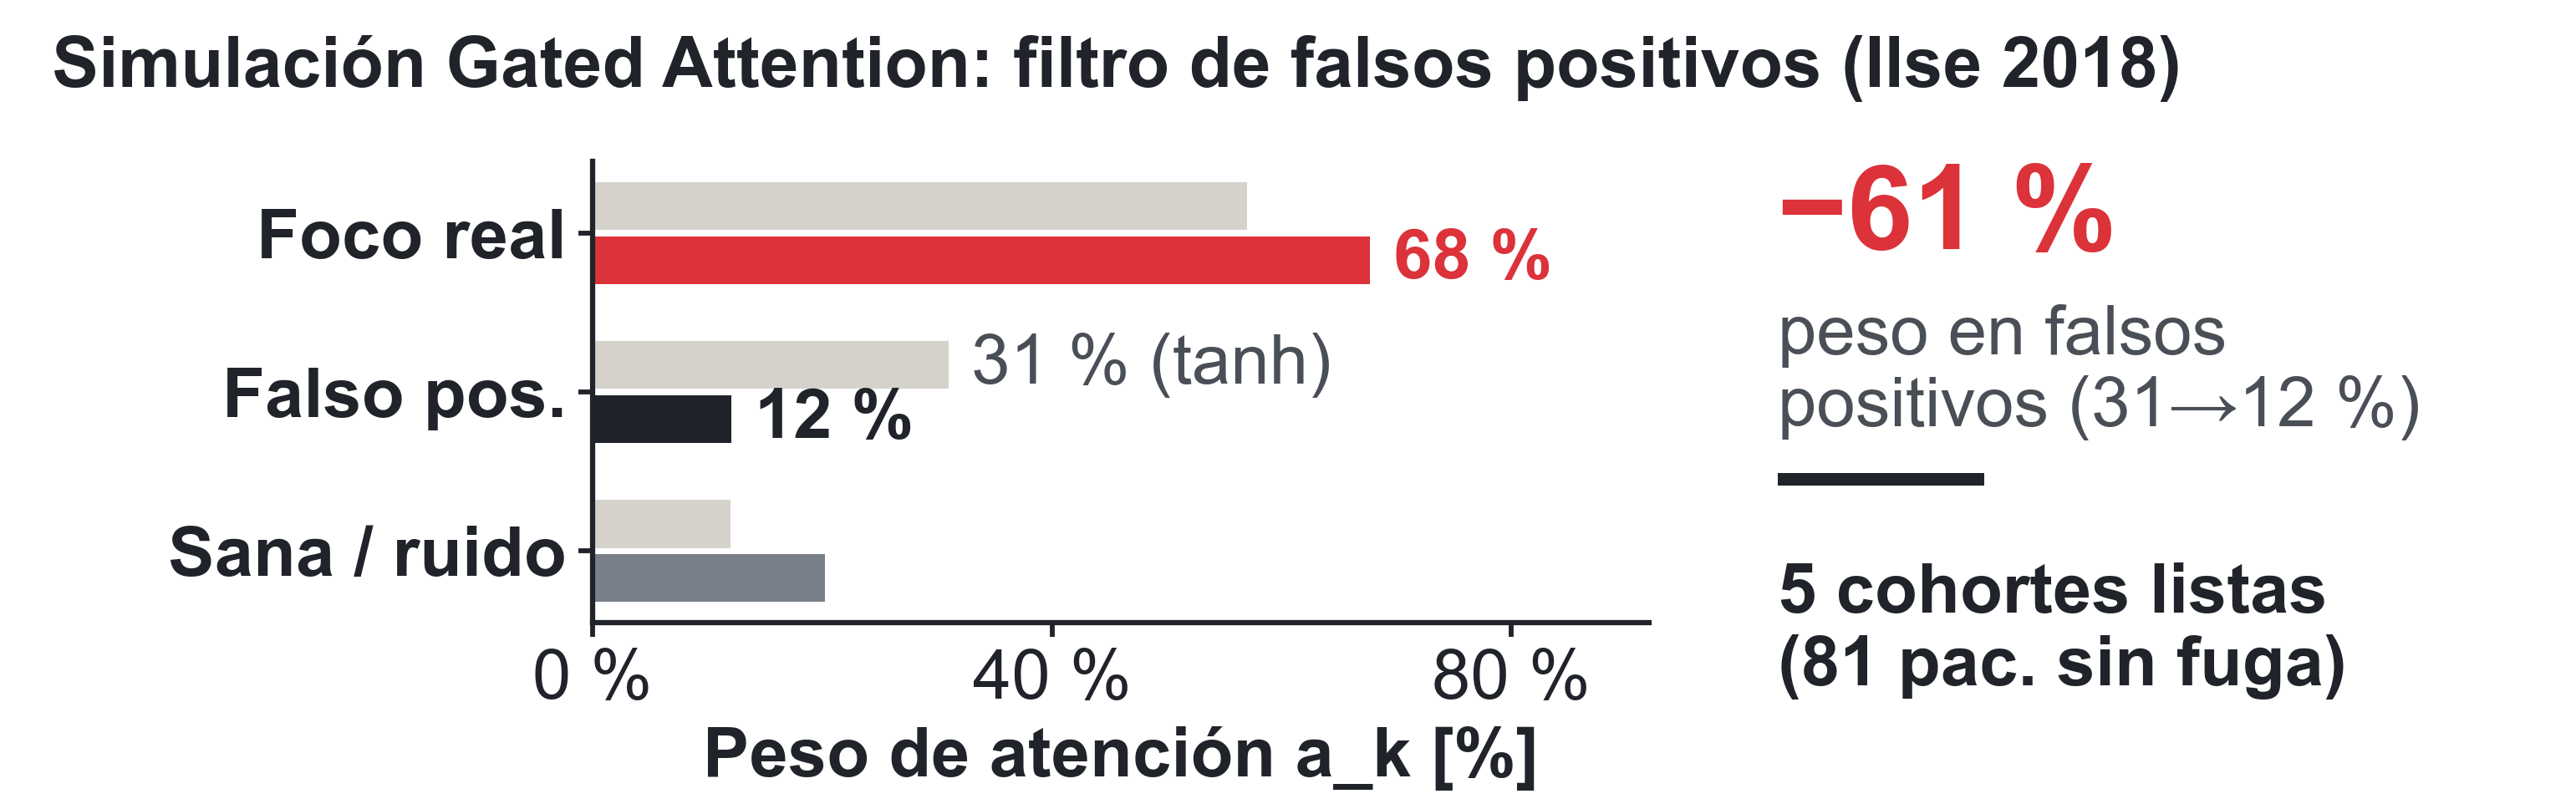
\includegraphics[width=26.10cm, height=8.20cm]{assets/fig4_avance.png}%
  };
  \node[anchor=north west, inner sep=0pt, text=udpink, text width=26.10cm] at (30.30, 60.60) {%
    \fsize{24}{29}\AvanceDetalle\par
  };

  \draw[udpline, line width=1.0pt] (3.00, 63.40) -- (56.40, 63.40);

  % ============================================================================
  % ZONA 3: PLAN DE TRABAJO (y = 63.40 .. 74.60 cm)
  % ============================================================================
  \fill[udpred] (3.00, 64.60) rectangle (4.60, 64.82);
  \node[anchor=north west, inner sep=0pt, text=udpred] at (3.00, 65.10) {%
    \fsize{20}{24}\bfseries Plan%
  };
  \node[anchor=north west, inner sep=0pt, text=udpink, text width=53.40cm] at (3.00, 66.15) {%
    \fsize{30}{35}\bfseries \PlanMensaje\par
  };
  \node[anchor=north west, inner sep=0pt] at (3.00, 68.20) {%
    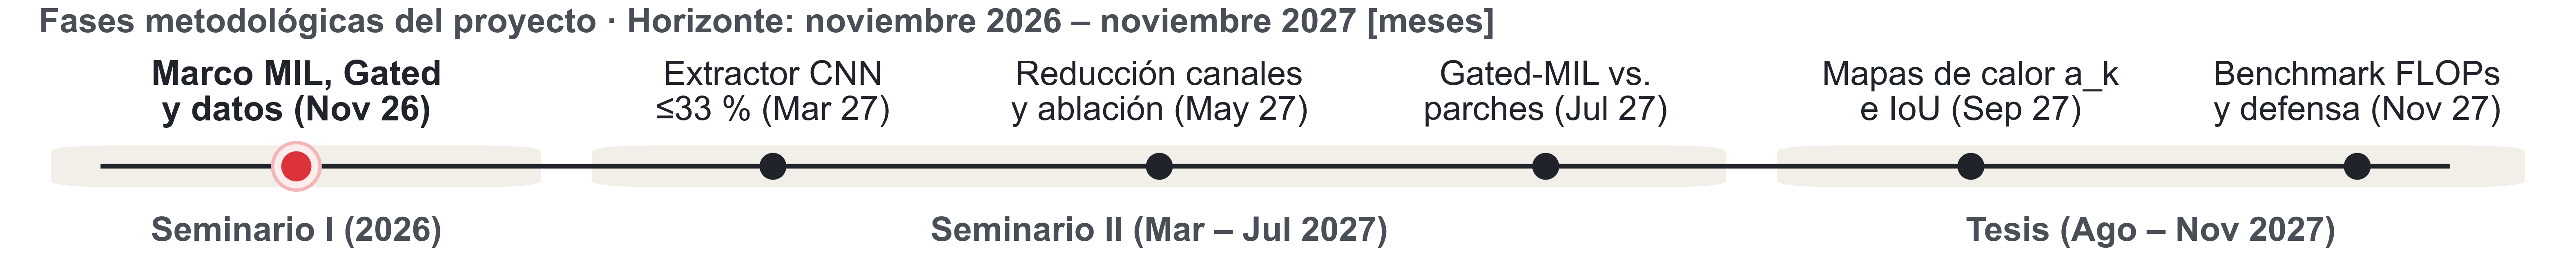
\includegraphics[width=53.40cm, height=5.40cm]{assets/fig5_plan.png}%
  };

  % ============================================================================
  % PIE OSCURO: PREGUNTAS DE RETROALIMENTACION Y CODIGO QR (y = 74.60 .. 84.10 cm)
  % ============================================================================
  \node[anchor=north west, inner sep=0pt, text=udpcoral] at (3.00, 75.70) {%
    \fsize{24}{28}\bfseries Busco retroalimentaci\'on sobre%
  };
  \node[anchor=north west, inner sep=0pt, text=white, text width=42.20cm] at (3.00, 76.95) {%
    \fsize{24}{31}1.\;\; \PreguntaUno\\[4pt]
    2.\;\; \PreguntaDos\par
  };

  % Leyenda y Codigo QR
  \node[anchor=east, inner sep=0pt, text=udpfootgray, align=right] at (51.55, 77.80) {%
    \fsize{16}{20}Referencias\\y art\'iculos\\consultados%
  };
  \fill[white, rounded corners=2pt] (52.00, 75.60) rectangle (56.40, 80.00);
  \node[anchor=north west, inner sep=0pt] at (52.30, 75.90) {%
    
\includegraphics[width=3.80cm, height=3.80cm]{assets/qr_referencias.png}%
  };

  \draw[white!22!udpfooter, line width=0.9pt] (3.00, 80.55) -- (56.40, 80.55);

  \node[anchor=north west, inner sep=0pt] at (3.00, 81.05) {%
    
\includegraphics[width=9.86cm]{assets/logo_posgrado_blanco.png}%
  };
  \node[anchor=north east, inner sep=0pt, text=udpfootgray, align=right, text width=42.50cm] at (56.40, 81.15) {%
    \fsize{16}{20}\PieEvento\\
    \PieFinanciamiento\par
  };

\end{tikzpicture}%
\end{document}
